\documentclass{article}

% if you need to pass options to natbib, use, e.g.:
%     \PassOptionsToPackage{numbers, compress}{natbib}
% before loading neurips_2019

% ready for submission
% \usepackage{neurips_2019}

% to compile a preprint version, e.g., for submission to arXiv, add add the
% [preprint] option:
%     \usepackage[preprint]{neurips_2019}

% to compile a camera-ready version, add the [final] option, e.g.:
\usepackage[final]{neurips_2019}
\setcitestyle{square}

% to avoid loading the natbib package, add option nonatbib:
    % \usepackage[nonatbib]{neurips_2019}

\usepackage[utf8]{inputenc} % allow utf-8 input
\usepackage[T1]{fontenc}    % use 8-bit T1 fonts
\usepackage[hidelinks]{hyperref}       % hyperlinks
\usepackage{url}            % simple URL typesetting
\usepackage{booktabs}       % professional-quality tables
\usepackage{amsfonts}       % blackboard math symbols
\usepackage{nicefrac}       % compact symbols for 1/2, etc.
\usepackage{microtype}      % microtypography
\usepackage{graphicx}  % <--- added
\usepackage{subcaption}

\makeatletter
\newcommand{\printfnsymbol}[1]{%
  \textsuperscript{\@fnsymbol{#1}}%
}
\makeatother

\title{Reproducibility Report - One ticket to win them all: generalizing lottery ticket initializations across datasets and optimizers}


\author{%
  Varun Gohil\thanks{Denotes equal contribution.} \\
  IIT Gandhinagar\\
  \texttt{gohil.varun@iitgn.ac.in} \\
  \And 
  S. Deepak Narayanan\printfnsymbol{*} \\
  IIT Gandhinagar\\
  \texttt{deepak.narayanan@iitgn.ac.in} \\
  \And
  Atishay Jain\printfnsymbol{*}\\
  IIT Gandhinagar\\
  \texttt{atishay.jain@iitgn.ac.in} \\
}

\begin{document}

\maketitle




\begin{abstract}
The lottery ticket hypothesis states that smaller subnetworks within a larger deep network can be trained in isolation to achieve accuracy similar to that of original network, as long as they are initialized appropriately. However, whether these subnetworks or winning tickets are transferable across datasets and optimizers remains unclear. The paper "One ticket to win them all:generalizing lottery ticket initializations across datasets and optimizers" empirically shows that these winning tickets are transferable. We reproduce the results in the paper from scratch by implementing all the experiments. 
Our results support the original paper's claim of the winning ticket initializations being transferable. While the paper is replicable, we find that reproducing the paper requires access to large amount of computing resources for generating the winning tickets. Hence we also open-source the winning tickets we find, so others can avoid the compute-intensive procedure of generating them.
\end{abstract}


\section{Introduction}
\label{sec:intro}
Prior works have shown that 90\% of the parameters of a neural network can be eliminated without compromising accuracy \cite{han_prune, ref2}. Eliminating unnecessary parameters by techniques like pruning reduces the computation requirements and energy consumption of neural networks thereby making inference more efficient. The procedure for pruning networks involves training the entire neural network and eliminating the least important weights after the training phase has been completed. However, if the number of parameters in a neural network can be reduced, why not train the pruned network itself and make training phase more efficient?

Pruned networks were not trained from scratch as previous works \cite{ref2, han_prune} mention that when pruned networks are trained from scratch they achieve lower accuracy when compared to a network which is pruned after training. However, the recently proposed lottery ticket hypothesis states the following:\\
\textit{"A randomly-initialized, dense neural network contains a subnetwork that is initialized such that—when trained in isolation—it can match the test accuracy of the original network after training for at most the same number of iterations"} \cite{lth_orig_paper}.
These subnetworks along with the appropriate initializations are referred to as the \textit{winning tickets}. If true, the lottery ticket hypothesis implies that pruned networks can be trained from scratch to achieve accuracy commensurate to the accuracy of original network as long as the pruned network is initialized appropriately. 

Unfortunately, finding these winning ticket initializations requires one to iteratively prune the network which is a computationally expensive procedure. One can potentially avoid this procedure if one can reuse the same winning ticket initialization across multiple datasets and optimizers. However, the answer to the question of whether these winning ticket initializations generalize to the spectrum of datasets and optimizers remains obscure. The paper we reproduce,  \textit{"One ticket to win them all: generalizing lottery ticket initializations across datasets and optimizers"} \cite{repro_paper} provides empirical evidence that these winning ticket initializations generalize across multiple datasets as well as optimizers\footnote{Authors used anywhere in this paper refers to the authors of the paper that we reproduce \cite{repro_paper}}.
 
 
As a part of the NeurIPS Reproducibility Challenge's \textit{Replication Track}, we replicate the work done by \cite{repro_paper} and investigate if the winning ticket initializations are generalizable across datasets and optimizers. The target questions of our work are as follows:
\begin{itemize}
    \item Do winning ticket initializations generalize within same data distribution?
    \item Do winning ticket initializations generalize across datasets?
    \item Do winning ticket initializations generalize across optimizers?
\end{itemize}

In this report, Section \ref{sec:method} describes the techniques we used for our experiments and their implementation.  Section \ref{sec:cost} describes the efforts needed to replicate the results in terms of computing resources required, development time and contact with authors. Further, in Section \ref{sec:results} we present and discuss our results. We open source the code we use for our experiments\footnote{The code base can be found at \href{https://github.com/varungohil/Generalizing-Lottery-Tickets}{\texttt{github.com/varungohil/Generalizing-Lottery-Tickets}}}. Finally, as finding these winning tickets is computationally expensive, we open-source the winning tickets we found for usage by the community\footnote{The winning tickets can be found in this  \href{https://drive.google.com/drive/folders/1Nd-J4EwmgWbUARYaqe9iCF6efEFf9S2P?usp=sharing}{\texttt{Google Drive folder}} (hyperlinked)}. 


\section{Methodology and Experimental Settings}
\label{sec:method}
We implement the code base using PyTorch \cite{pytorch}. We use the inbuilt model definitions, optimizers, datasets of PyTorch for our experimentation.

\subsection{Models}
\label{subsec:models}
For all our experiments, we use one of the two network  architectures: ResNet50 and a modified VGG19. 

In the case of the modified VGG19 architecture, we remove all the fully connected layers from the network. Following the last convolutional layer, we add a global-average-pooling layer. Finally, we add a linear classification layer from the global average pool to the number of output classes. We use the ReLU non-linearity and perform batch normalization after each convolutional layer. For our experiments, we initialize all the convolutional layers using Xavier normal initialization and the biases to 0. We set batch norm weights and bias parameters to 1 and 0 respectively. We train all the VGG19 models for 160 epochs and anneal the learning rates
by a factor of 10 at the 80$^{th}$ and the 120$^{th}$ epochs. 

We use the standard ResNet50 architecture that was proposed in \cite{DBLP:journals/corr/HeZRS15}. We use the Kaiming normal initialization for convolutional layers, which is also the default initialization for ResNets in PyTorch. We train all the ResNet models for 90 epochs. We anneal the learning rates by a factor of 10 at the 50$^{th}$, 65$^{th}$ and 80$^{th}$ epochs. 

The initializations, number of epochs, learning rate annealing schedules are in accordance to \cite{repro_paper} to maintain consistency of experiments.

\subsection{Optimizers}
We used two optimizers for our experiments - The Adam optimizer and Stochastic Gradient Descent (SGD) optimizer. We use Adam with a learning rate of 0.0003 with betas 0.9 and 0.999 and a weight decay of 0.0001. We use SGD with a learning rate of 0.1, with a momentum of 0.9 and a weight decay of 0.0001. We use hyperparameters provided by authors to maintain consistency with the paper we are reproducing \cite{repro_paper}.

\subsection{Datasets}
We use 4 datasets for our experiments - CIFAR10 \cite{cifar}, CIFAR100 \cite{cifar}, SVHN \cite{svhn} and FashionMNIST \cite{fashionmnist}. These datasets are diverse in terms of grayscale vs. color images, input size, number of output classes,
and training set size. For all these datasets for data augmentation we perform random horizontal flips and random crops of size 32 with a padding of 4. We use the default train-test splits provided by PyTorch dataloaders in our experiments. We use a batch size of 512 for all our experiments. 


\subsection{Pruning Methodology and Implementation}
There are two widely used methods for pruning - one shot pruning and iterative pruning. Suppose we want to prune $p\%$ of a network.  In one shot pruning, we first train the network, then prune $p\%$ of the weights and finally reset the weights to the original initialization that the network had before training. In iterative pruning the network is trained, pruned and reset every round for $n$ rounds. As can be observed, at the end of each round, $p^{\frac{1}{n}} \%$ of the weights that survived the previous round are pruned. In this work we use iterative pruning for pruning the neural networks.  We use iterative pruning as prior work \cite{lth_orig_paper} shows that it finds winning tickets that match the accuracy of original network at higher pruning fractions when compared to one shot pruning.

Further, for each iteration a neural network can be pruned either in a global manner or in a local manner. When pruning in a global manner, the weights of all layers of the network are pooled together and then a fraction of weights are removed from this global pool. In local pruning, the same fraction of weights are removed in each layer for all the layers. In our work we use global pruning as used in the paper we are reproducing \cite{repro_paper}.

In our implementation of pruning,  we set the value of the parameters to be pruned to be zero before each forward pass by multiplying the parameter tensor with a binary mask of identical shape. This automatically ensures two things: (a) the forward pass is on the pruned network and (b) the gradients are computed on the pruned network. 

We perform iterative pruning for 30 pruning iterations and use a 20\% pruning rate. For our experiments we use magnitude-based pruning i.e. the weights with the magnitudes in the lowest 20\% of remaining non-zero weights are removed after each iteration. 


\subsection{Late Resetting}
In the original paper on lottery ticket hypothesis \cite{lth_orig_paper}, the authors reset the weights after each pruning iteration to the original initialization that the network had before training. They report that learning rate warm-up is necessary to find winning tickets on larger models. However, a recent work  \cite{DBLP:journals/corr/abs-1903-01611}, reports that re-initializing the weights to the weights after the training iteration $k$, where $k$ is typically much smaller than the total training iterations, performs consistently better in producing winning tickets and also removes the need for learning rate warm-up. We employ late resetting of 1 epoch in all the experiments as used by the authors \cite{repro_paper}.



\subsection{Random Masks}
Winning tickets, contain information about two key aspects of the subnetwork: the structure of the sparse neural network as well as the initialization of the parameters. The structure of the subnetwork is stored in form of a mask which is a binary vector that is multiplied with the network's weights, to set the pruned weights to zero. Prior works have preserved the structure of the mask while randomly initializing the weights for random tickets. The authors \cite{repro_paper} empirically demonstrate that the structure of the subnetwork contains significant information. Hence for the random ticket the authors apply a random mask to the network and initialize the parameters randomly. For implementing the random ticket baseline, we generate random masks by globally permuting the winning masks as mentioned in \cite{repro_paper}. 



\subsection{Computing Resources}
We run our experiments on three GPUs - Nvidia P100, Nvidia K80 and Nvidia GTX 1080. The Nvidia P100 and Nvidia K80 machines had a 16 core Intel processor and 15GB RAM, while the Nvidia GTX 1080 machine had a 32 core Intel processor with 256 GB of RAM.







\section{Cost of Reproducibility}
\label{sec:cost}
The authors of the original paper \cite{repro_paper} did not release their code. We replicate the results by implementing the all experiments from scratch. We did not experience significant difficulty in developing the code base we use for our experiments. We believe that a person having experience with PyTorch  can implement the code without major challenges. Further, we also contacted the authors via email. We inquired about the data-augmentations used while training the networks as they were not mentioned in the original paper. Further we contacted them to understand the concept of random masks. 

Replicating the results required a significant amount of computing resources. We experienced that the CodeOcean compute resources provided by organizers of NeurIPS Reproducibility Challenge,  were not sufficient for the experimentation and hence we performed the experiments on Google Cloud. Further, finding winning tickets for larger datasets is computationally expensive, with the authors using 16 GPUs \cite{repro_paper}. As we did not have access to such a large amount of computing resources, we only replicated the results on smaller datasets like Cifar-10, Cifar-100, SVHN and FashionMNIST. We could not conduct experiments for larger datasets like ImageNet (1.8 million images) \cite{imagenet} and Places365 (8 million images) \cite{places365} as we were severely limited by compute capability and the time allotted for the reproducibility challenge. Overall, we used  approximately \$500 worth of Google Cloud credits for our experimentation.

The process of generating winning tickets is time-consuming as well. Training a ResNet50 model for 90 epochs using Nvidia P100, the fastest GPU we used, takes approximately 33 minutes. Similarly, training the VGG19 model for 160 epochs using Nvidia P100 takes approximately 43 minutes. For our experiments we trained a ResNet50 model 450 times and a VGG19 model 540 times. All the experiments would take approximately 634 hours (26 days) to run sequentially. To complete the experiments in time we scheduled multiple experiments parallelly on Google Cloud.  

We open-source our code base for reproducing the results of \cite{repro_paper}. Along with our code base, we also open-source the winning tickets we found during our experimentation. We hope this will help the community avoid expensive and time-consuming computation, as these winning tickets can directly be used for inference and can be studied to improve our understanding of lottery tickets. 

\section{Results and Discussion}
\label{sec:results}
The original paper reports results for 3 experiments, each concerning a target question we mentioned in Section \ref{sec:intro}. For each experiment, we plot the test accuracy at convergence as function of fraction of pruned weights. Owing to the compute and time constraints mentioned in Section \ref{sec:cost}, we could only replicate the results with 1 random seed. 

\subsection{Transfer within same data distribution}
With this experiment, we aim to investigate if the winning ticket initializations generalize within the same data distribution. For this experiment, we divide the CIFAR-10 dataset into 2 halves - CIFAR-10a and CIFAR-10b. Both these halves contain 25,000 training images, having 2500 images of each class. We find the winning ticket initialization for CIFAR-10a using SGD and verify if it generalizes to CIFAR-10b. As our baselines, we use the CIFAR-10b winning ticket initialization with SGD and random tickets. We perform this experiment for both, VGG19 and ResNet50 architectures,

  
\begin{figure}[h]
    \centering
    \begin{minipage}{.497\textwidth}
    \centering
    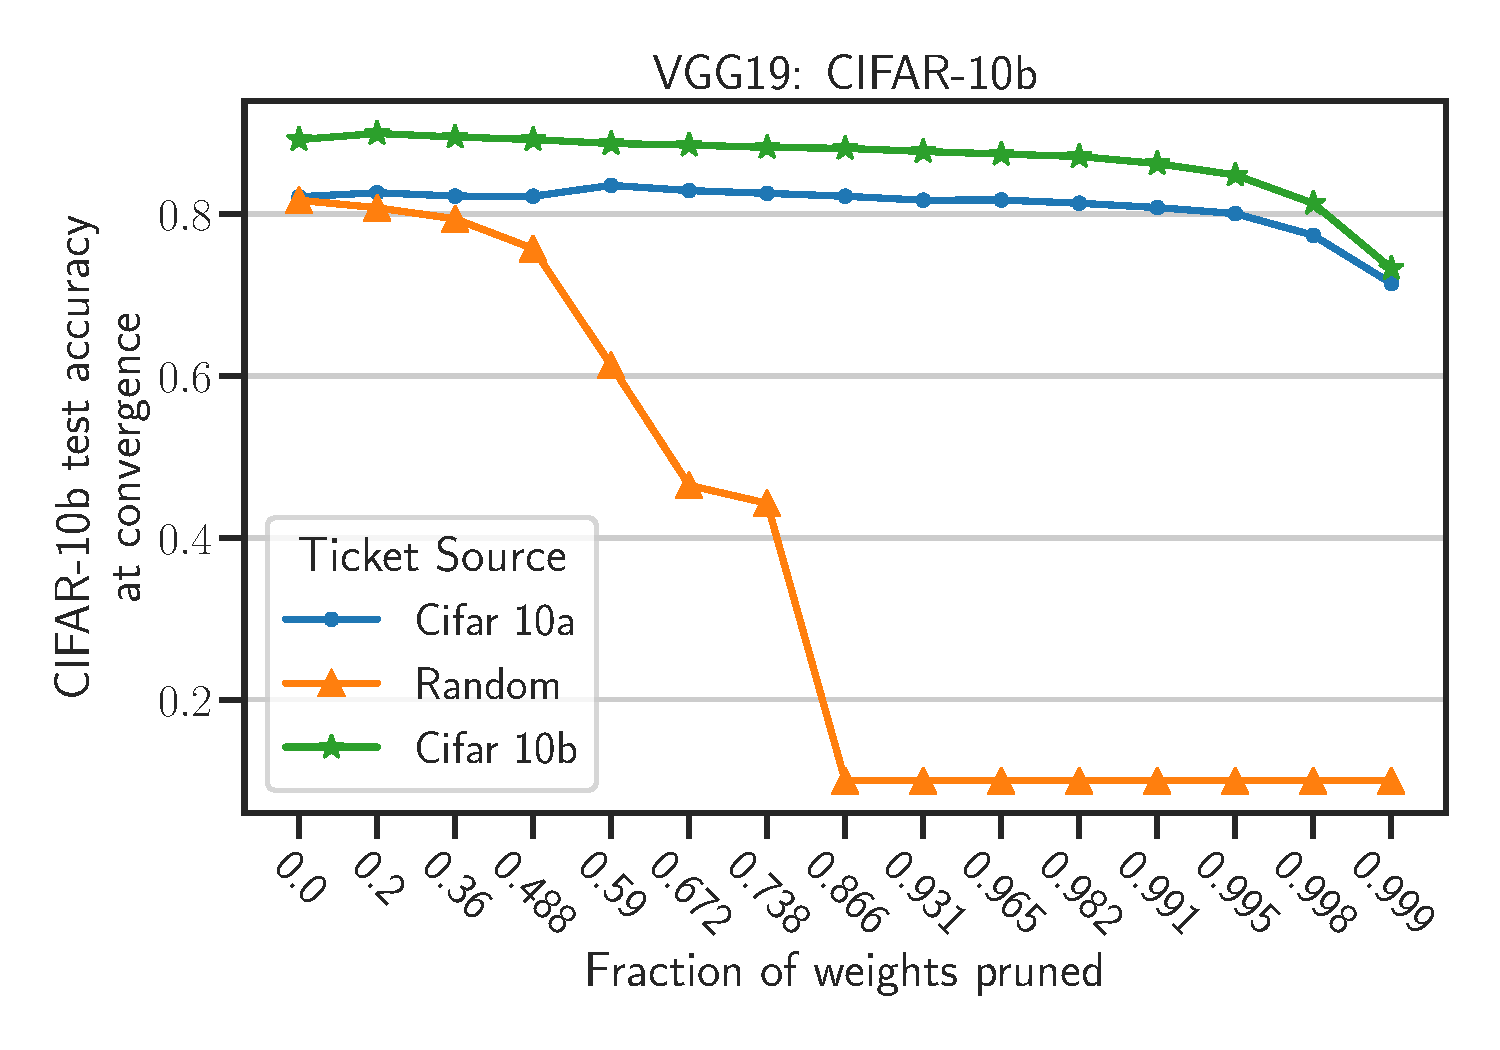
\includegraphics[width=\textwidth]{plots/Exp1_VGG_N.pdf}
    % \caption{Transfer of winning ticket initializations within same dataset using VGG19}
    % \label{fig:exp1_vgg}
    \end{minipage}
% \end{figure}
% \begin{figure}[h]
    % \centering
    \begin{minipage}{.497\textwidth}
    \centering
    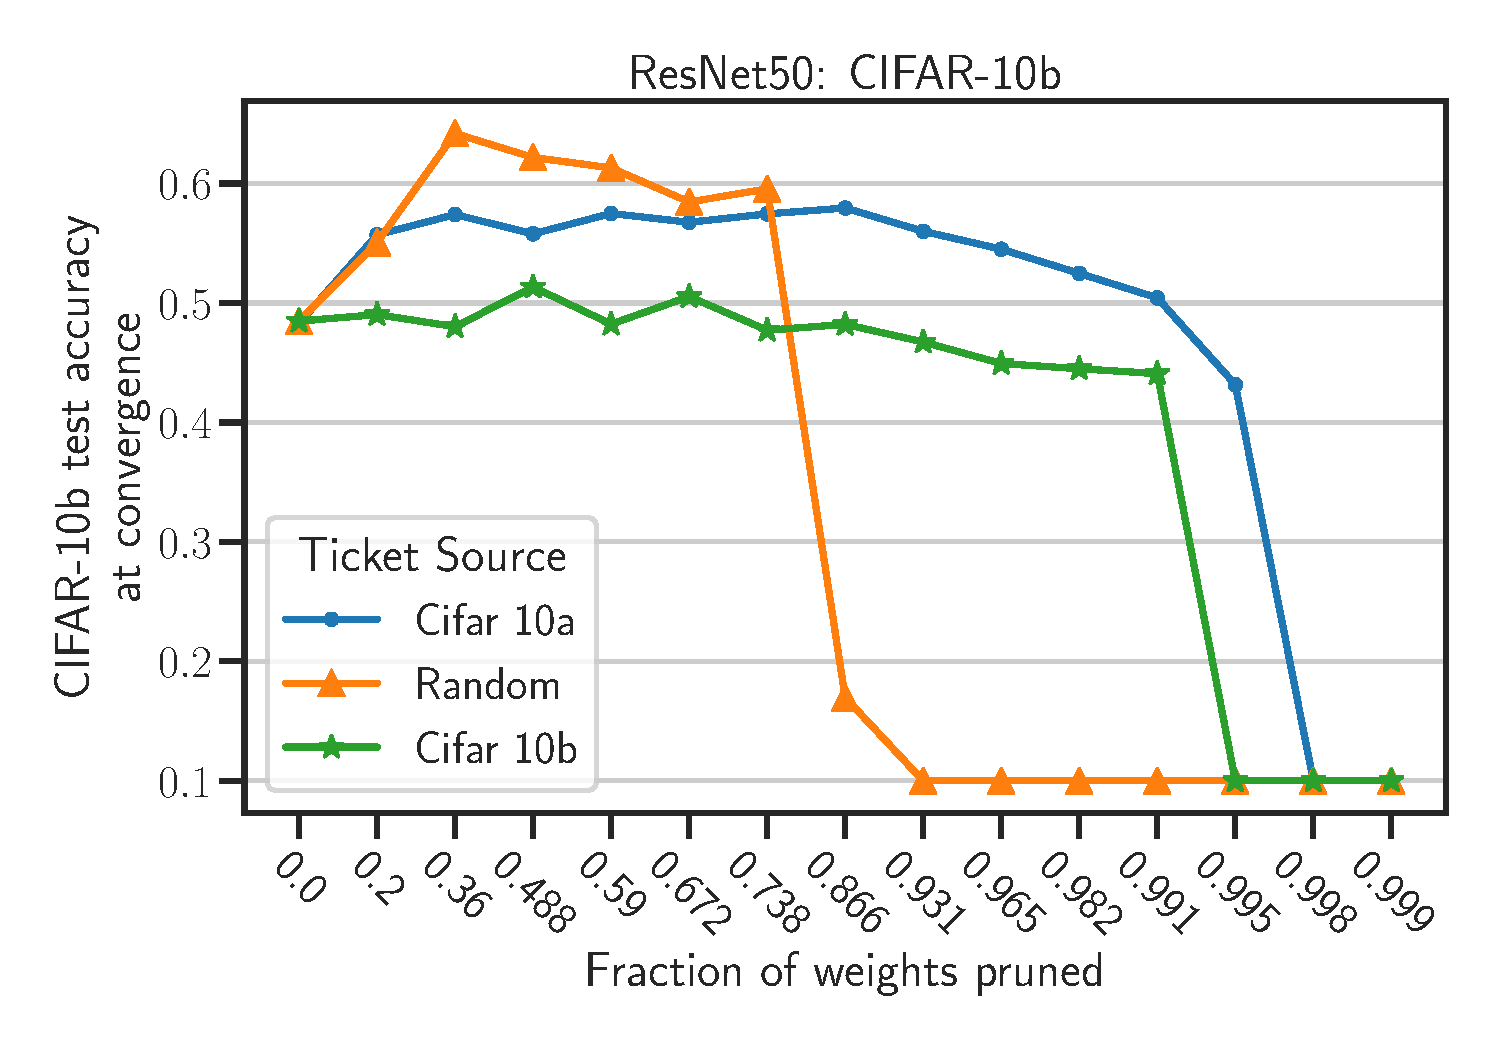
\includegraphics[width=\textwidth]{plots/Exp1_ResNet_N.pdf}
    % \caption{Transfer of winning ticket initializations within same dataset using ResNet50}
    % \label{fig:exp1_resnet}
    \end{minipage}
    \caption{Transfer of winning ticket initializations within same data distribution}
    \label{fig:exp1}
\end{figure}


Our results are presented in Figure \ref{fig:exp1}. The results show that winning tickets found on CIFAR-10a generalize well to CIFAR-10b. We also see that while using ResNet50, for low pruning fractions random ticket provides better accuracy than winning tickets found using CIFAR10-a and CIFAR10-b. The same phenomena is reported in the original paper \cite{repro_paper}. Our results support the hypothesis presented in original paper that ResNet50 winning tickets are sensitive to smaller datasets at low pruning fractions.


\subsection{Transfer across optimizers}
With this experiment, we aim to investigate if the winning ticket initializations generalize across optimizers. For our experiments, we use the modified VGG19 architecture discussed in Section \ref{subsec:models}. We find the winning tickets for CIFAR-10 dataset using both Adam and SGD optimizers and analyze the effect on accuracy when the ticket generated using one optimizer is further trained using another optimizer. Our results show that even after transfering tickets from SGD to Adam and vice-versa the accuracy of the tickets was comparable to when the tickets were trained using the same optimizer without any transfer. This supports the claim made in the original paper that VGG19 winning tickets are \textit{optimizer-independent}. 



\begin{figure}[h]
    \centering
    \begin{minipage}{.497\textwidth}
    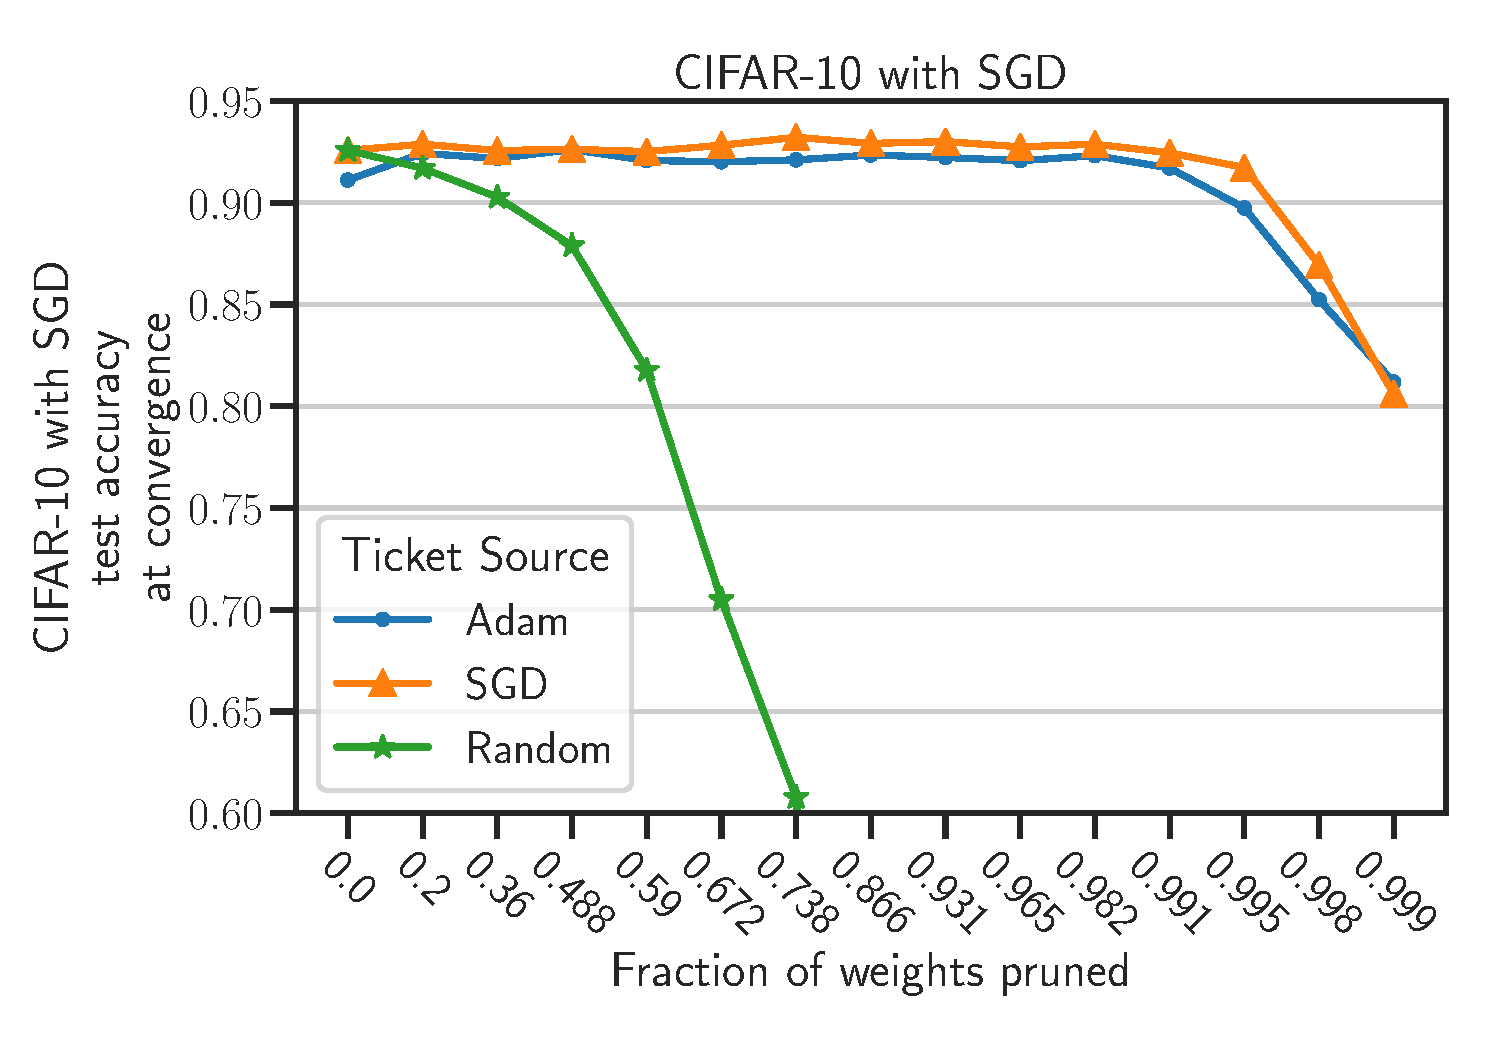
\includegraphics[width=\textwidth]{plots/Exp3_CIFAR10_SGD_N.pdf}
    % \caption{Transfer of winning ticket initializations across optimizers on SGD}
    % \label{fig:exp3_sgd}
    \end{minipage}
% \end{figure}
% \begin{figure}[h]
%     \centering
    \begin{minipage}{.497\textwidth}
    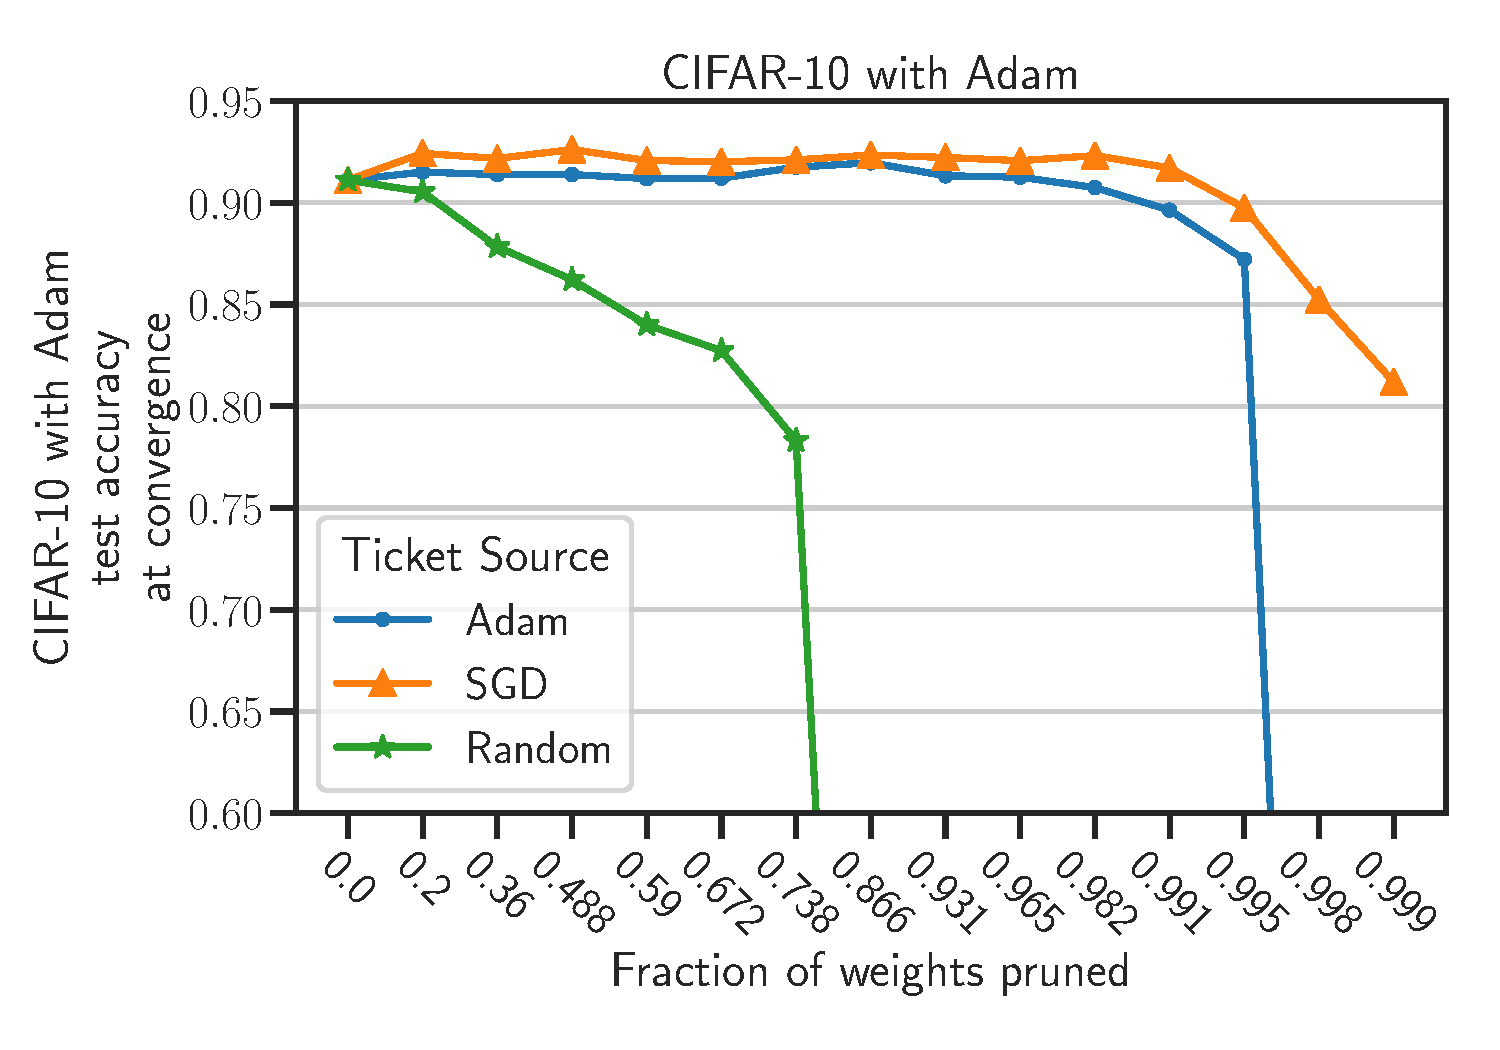
\includegraphics[width=\textwidth]{plots/Exp3_CIFAR10_Adam_N.pdf}
    % \caption{Tranfer of winning ticket initializations across optimizers on Adam}
    % \label{fig:exp3_adam}
    \end{minipage}
    \caption{Transfer of winning ticket initializations across optimizers}
    \label{fig:exp3}
\end{figure}

\subsection{Transfer across datasets}
With this experiment, we aim to investigate if the winning ticket initializations generalize across datasets. For our experiments, we used ResNet50 and the modified VGG19 architectures. We train the models on Cifar-10, Cifar-100, FashionMNIST and SVHN datasets with SGD optimizer. 

Our results also reveal the key trends which the authors discuss in the original paper. Firstly, we see in Figures \ref{fig:exp2_resnet} and \ref{fig:exp2_vgg} that individual winning tickets show accuracy similar to that of winning ticket generated on the target dataset. This supports the author's hypothesis that the inductive bias provided by the winning tickets is \textit{dataset-independent}.  

Second, we observe that winning tickets generated from more complex datasets (with higher number of classes) generalize better than those generated on relatively simpler datasets. Winning tickets generated on CIFAR-100 transfer better than those generated by those on CIFAR-10. This effect can be clearly seen in Figure \ref{fig:exp2_resnet} for ResNet50 architecture, while for VGG19 architecture both winning tickets show similar accuracy.

Third, while we observe that the winning rates transferred similarly for both ResNet50 and VGG19 architectures, the ResNet50 architecture tickets showed a sharper degradation in accuracy at higher pruning fractions compared to VGG19 architecture tickets. This can be observed by comparing Figure \ref{fig:exp2_resnet} with Figure \ref{fig:exp2_vgg}.

We do not report the results of VGG19 winning tickets on FashionMNIST as we exhausted our Google Cloud Credits before completion of the experiment. 

\begin{figure}[h]
    \centering
    \begin{minipage}{.497\textwidth}
    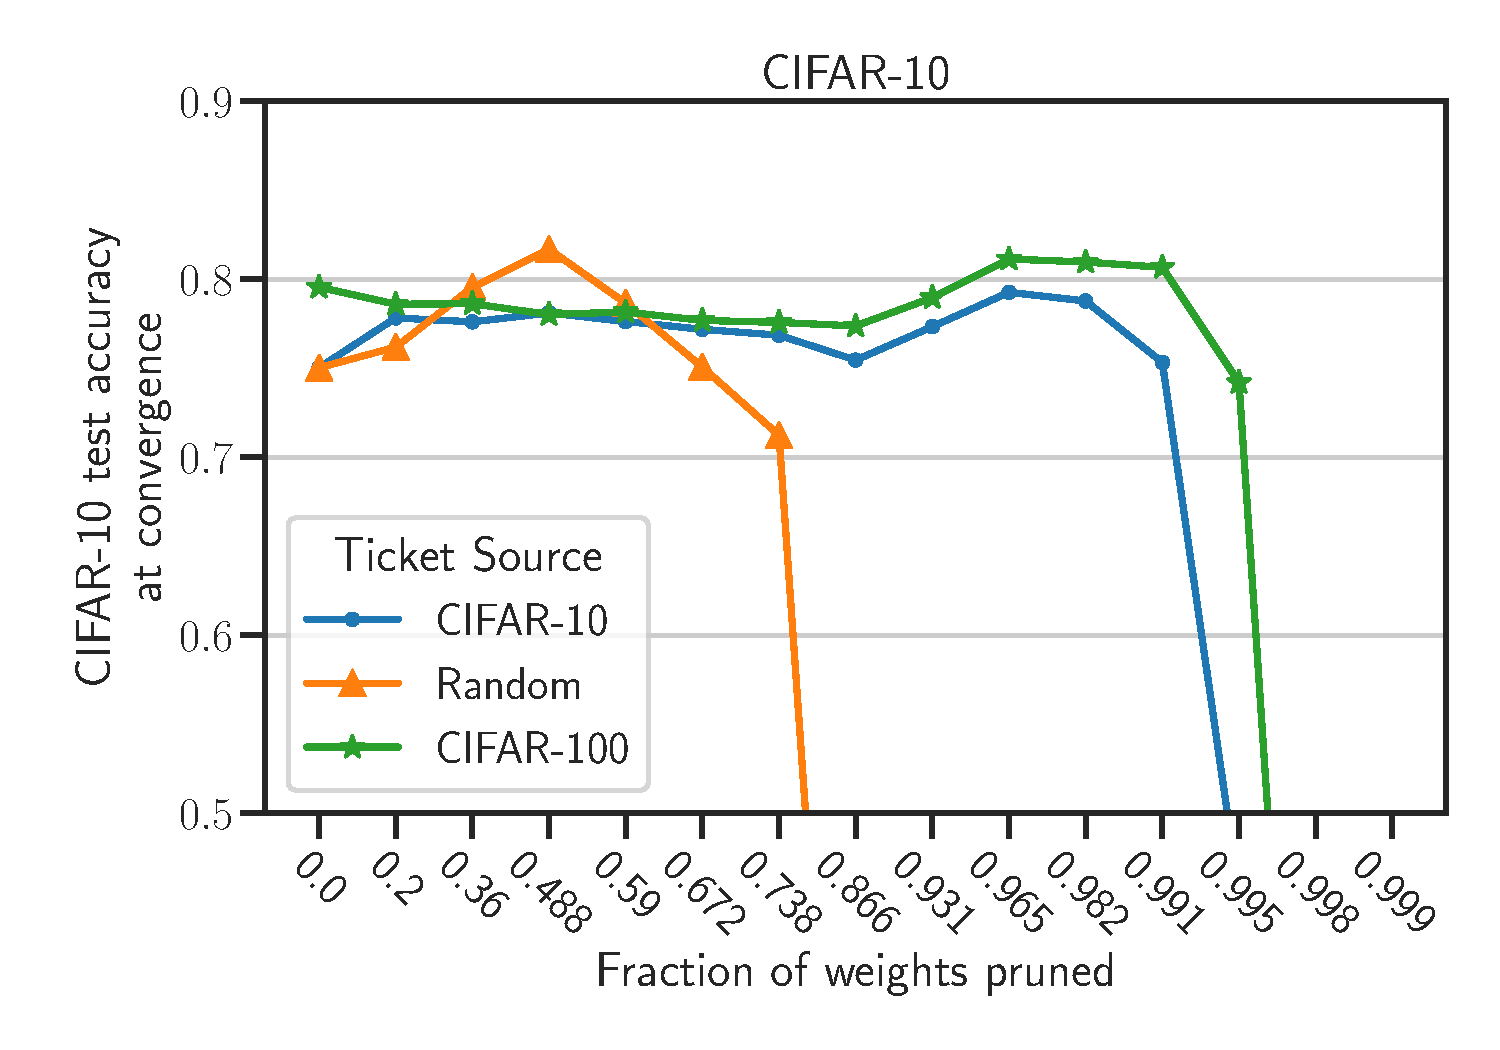
\includegraphics[width=\textwidth]{plots/Exp2_ResNet_CIFAR10_N.pdf}
    % \caption{Verifying transfer of winning ticket initializations across datasets - CIFAR10 with ResNet50}
    % \label{fig:exp2_resnet_cifar10}
    \end{minipage}
% \end{figure}
% \begin{figure}[h]
%     \centering
    \begin{minipage}{.497\textwidth}
    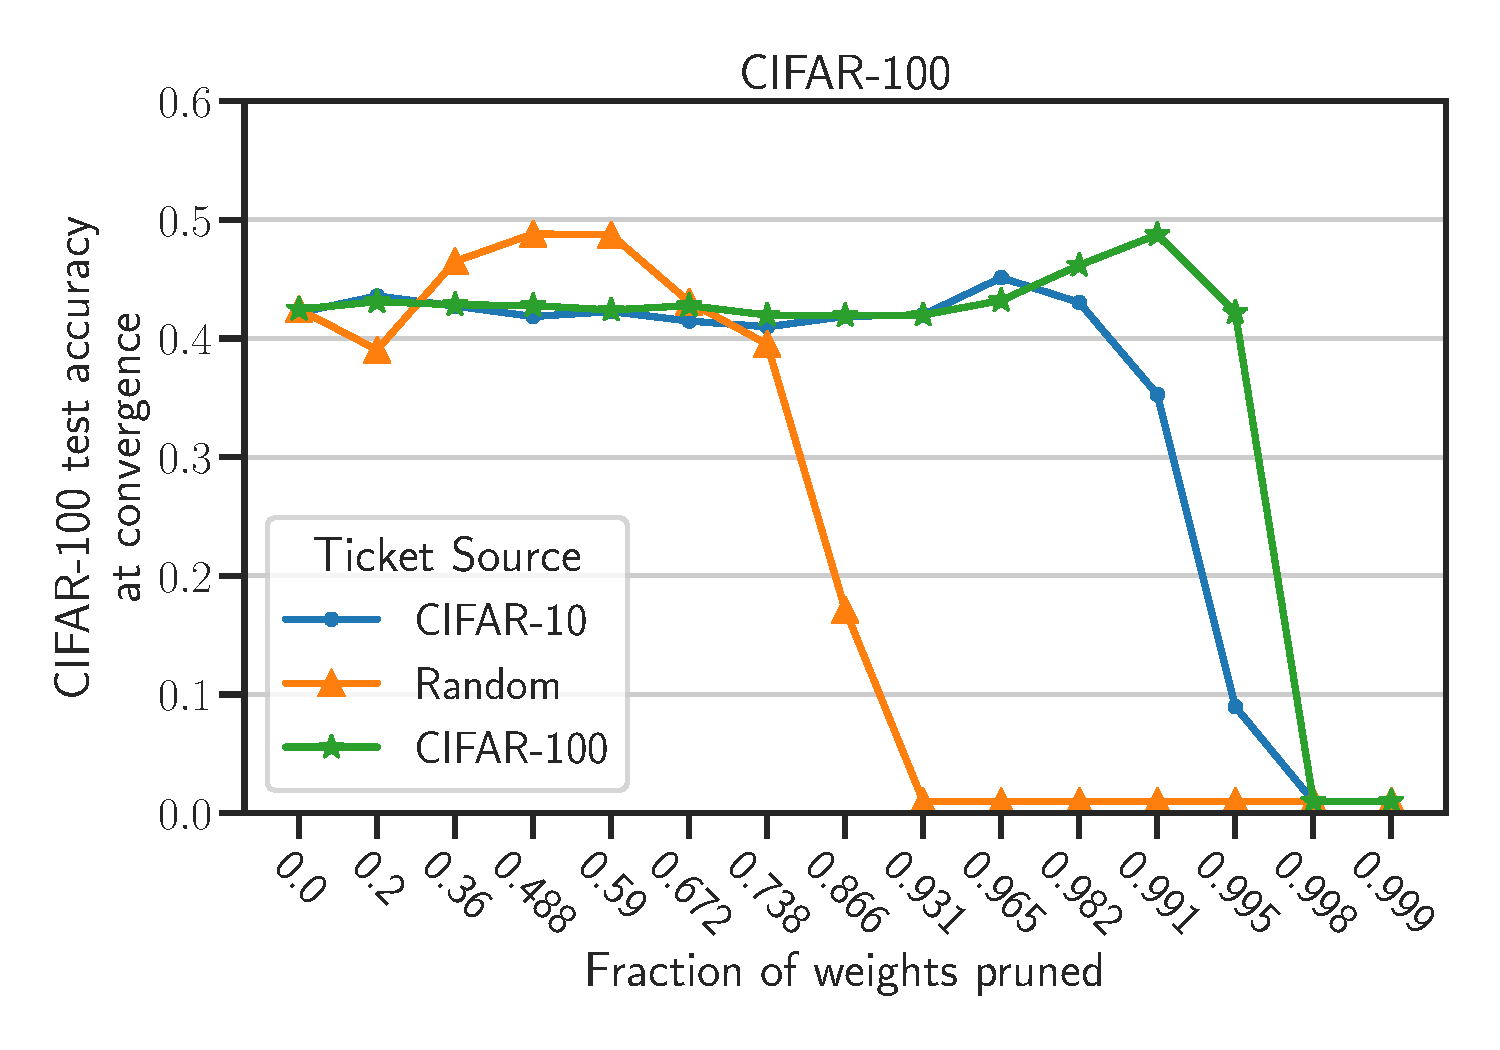
\includegraphics[width=\textwidth]{plots/Exp2_ResNet_CIFAR100_N.pdf}
    % \caption{Verifying transfer of winning ticket initializations across datasets - CIFAR100 with ResNet50}
    % \label{fig:exp2_resnet_cifar100}
    \end{minipage}
    % \caption{Transfer of winning ticket initializations across datasets with ResNet50}
    % \label{fig:exp2_resnet_1}
% \end{figure}
% \begin{figure}[h]
%     \centering
    \begin{minipage}{.497\textwidth}
    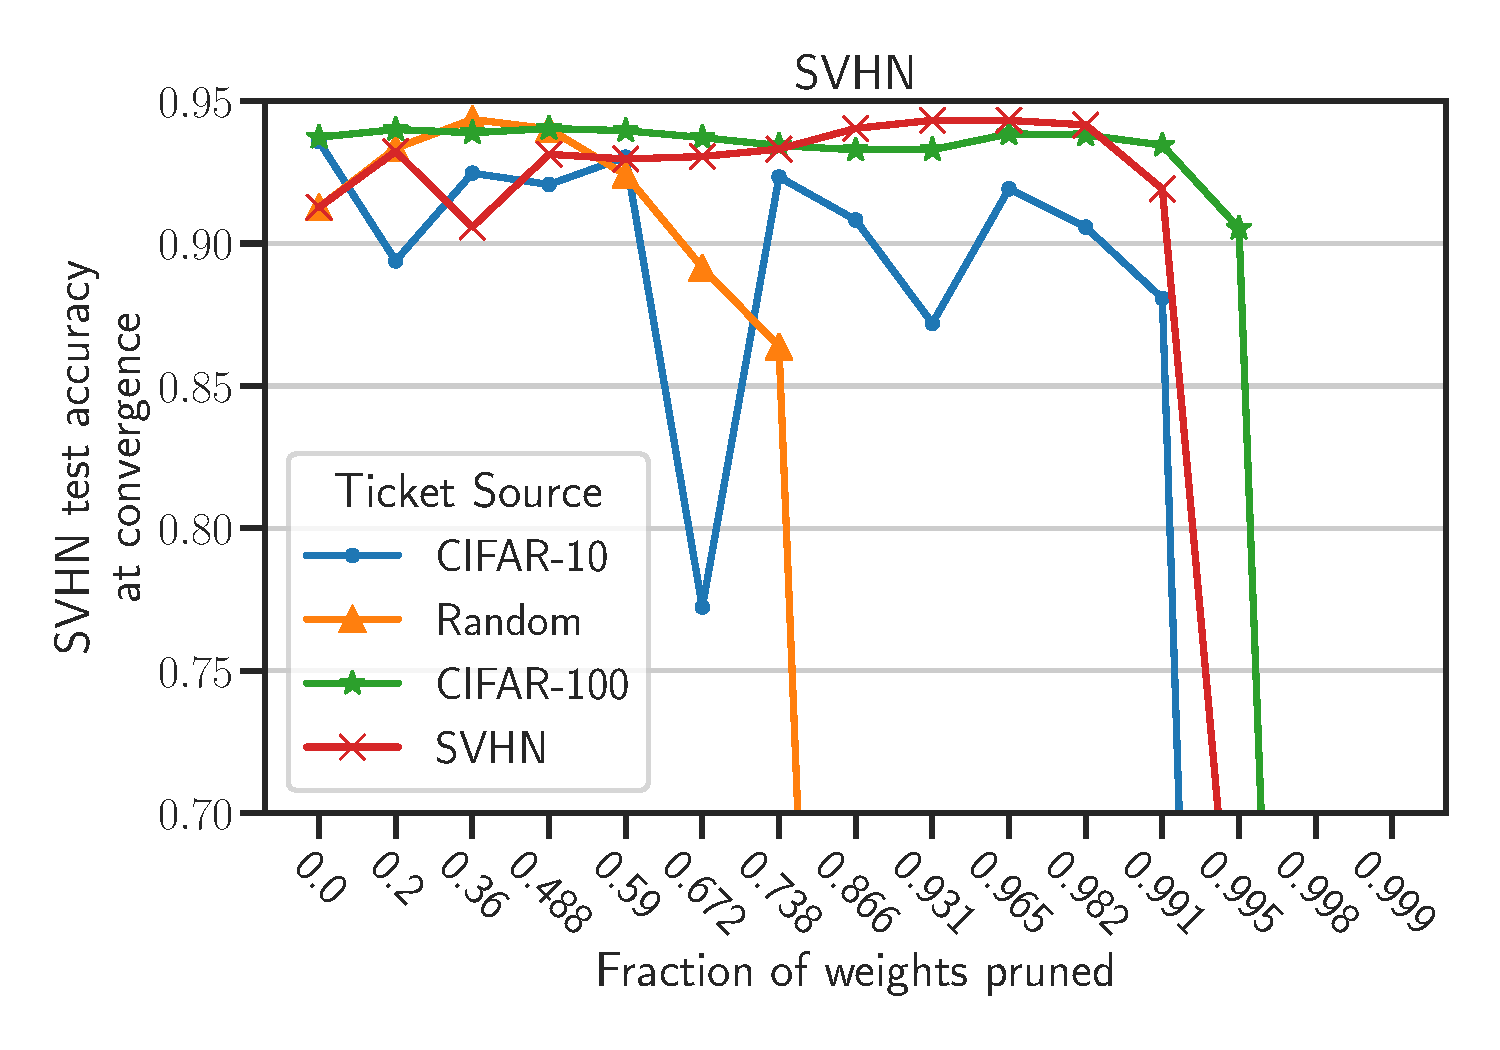
\includegraphics[width=\textwidth]{plots/Exp2_ResNet_SVHN_N.pdf}
    % \caption{Verifying transfer of winning ticket initializations across datasets - SVHN with ResNet50}
    % \label{fig:exp2_resnet_svhn}
    \end{minipage}
% \end{figure}
% \begin{figure}[h]
%     \centering
    \begin{minipage}{.497\textwidth}
    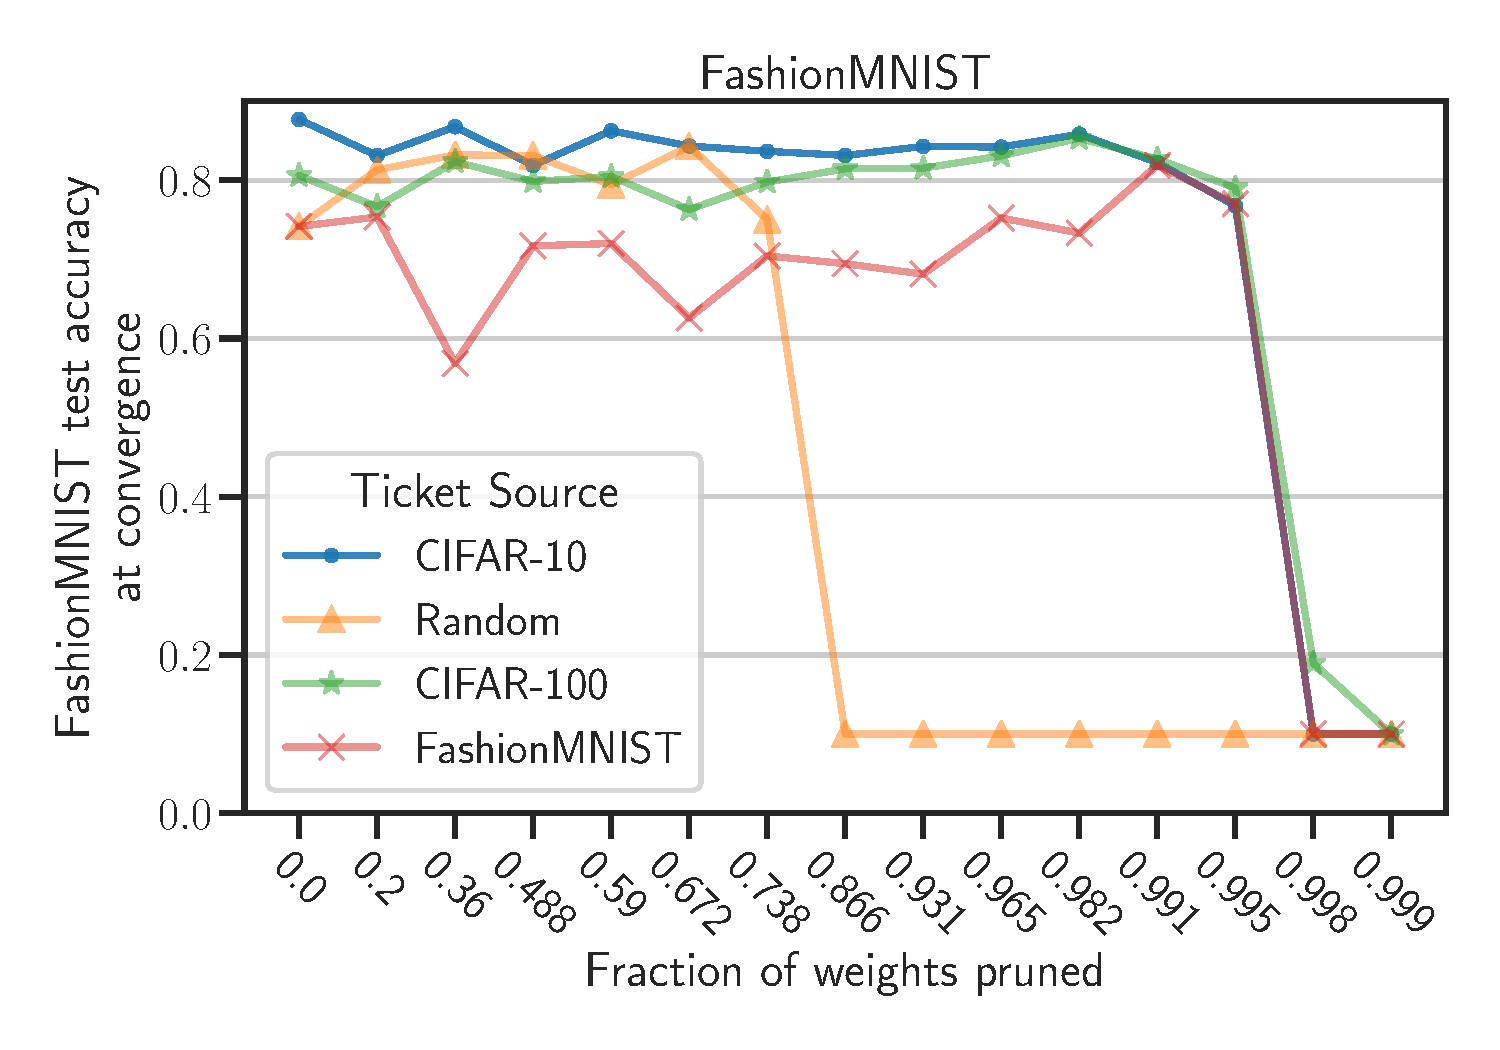
\includegraphics[width=\textwidth]{plots/Exp2_Resnet_FashionMNIST1_N.pdf}
    % \caption{Verifying transfer of winning ticket initializations across datasets - FashionMNIST with ResNet50}
    % \label{fig:exp2_resnet_fashionmnist}
    \end{minipage}
    \caption{Transfer of winning ticket initializations across datasets with ResNet50}
    \label{fig:exp2_resnet}
\end{figure}
\begin{figure}[]
    \centering
    \begin{minipage}{.497\textwidth}
    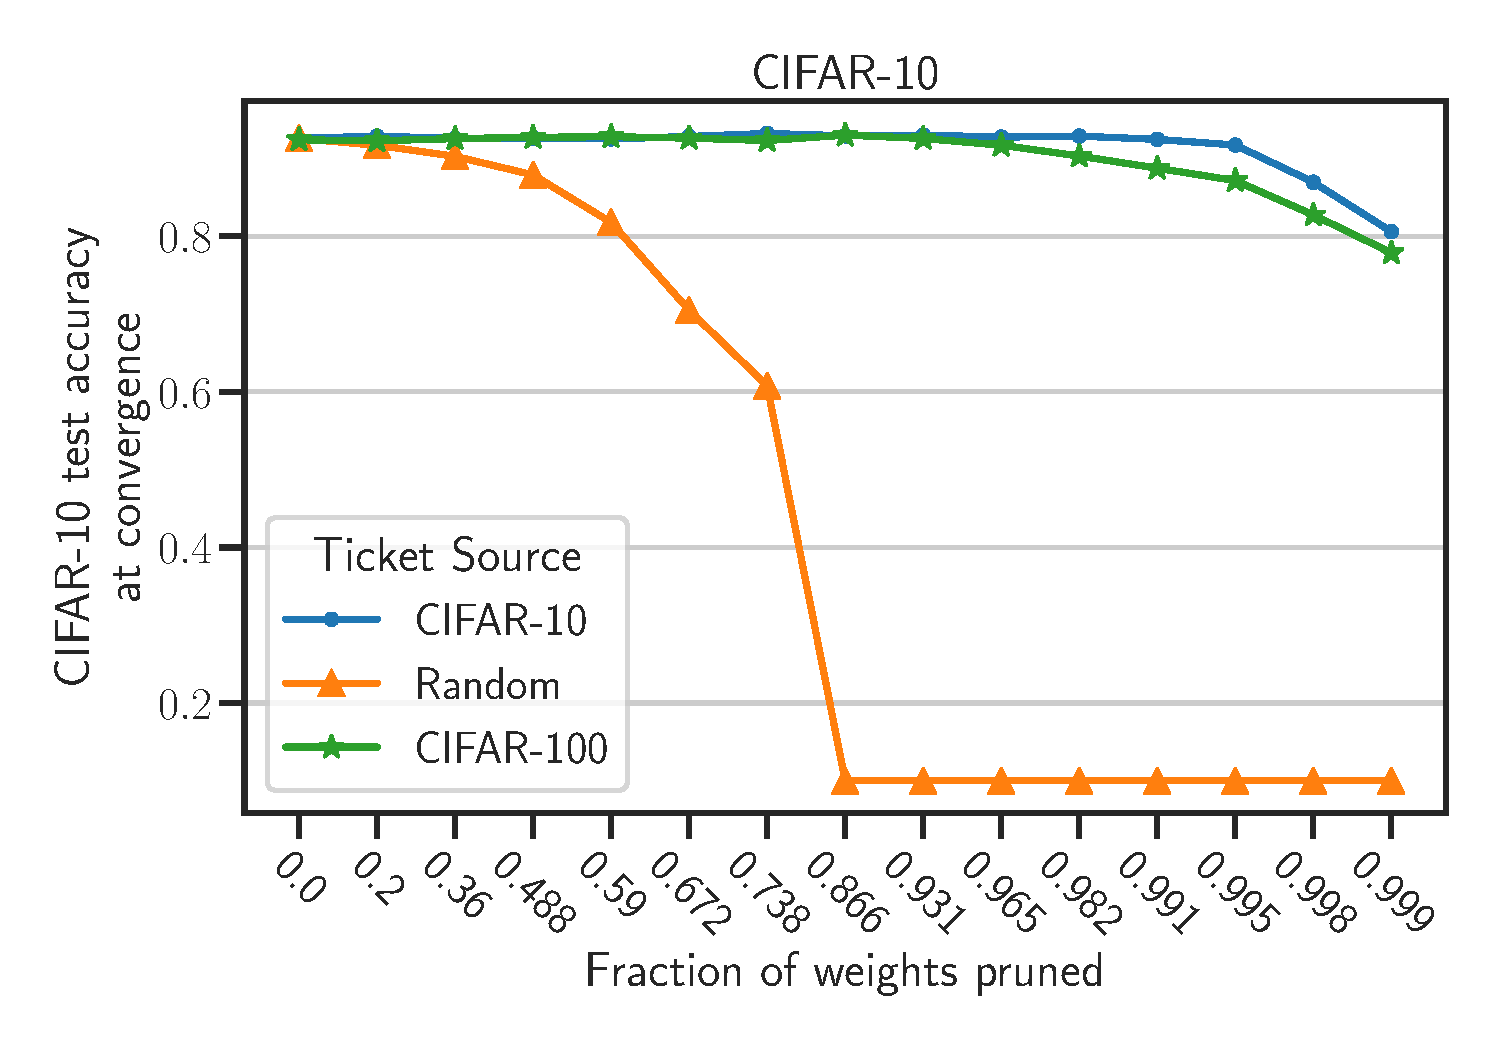
\includegraphics[width=\textwidth]{plots/Exp2_VGG_CIFAR10_N.pdf}
    % \caption{Verifying transfer of winning ticket initializations across datasets - CIFAR10 with VGG19}
    % \label{fig:exp2_vgg_cifar10}
    \end{minipage}
% \end{figure}
% \begin{figure}[h]
%     \centering
    \begin{minipage}{.497\textwidth}
    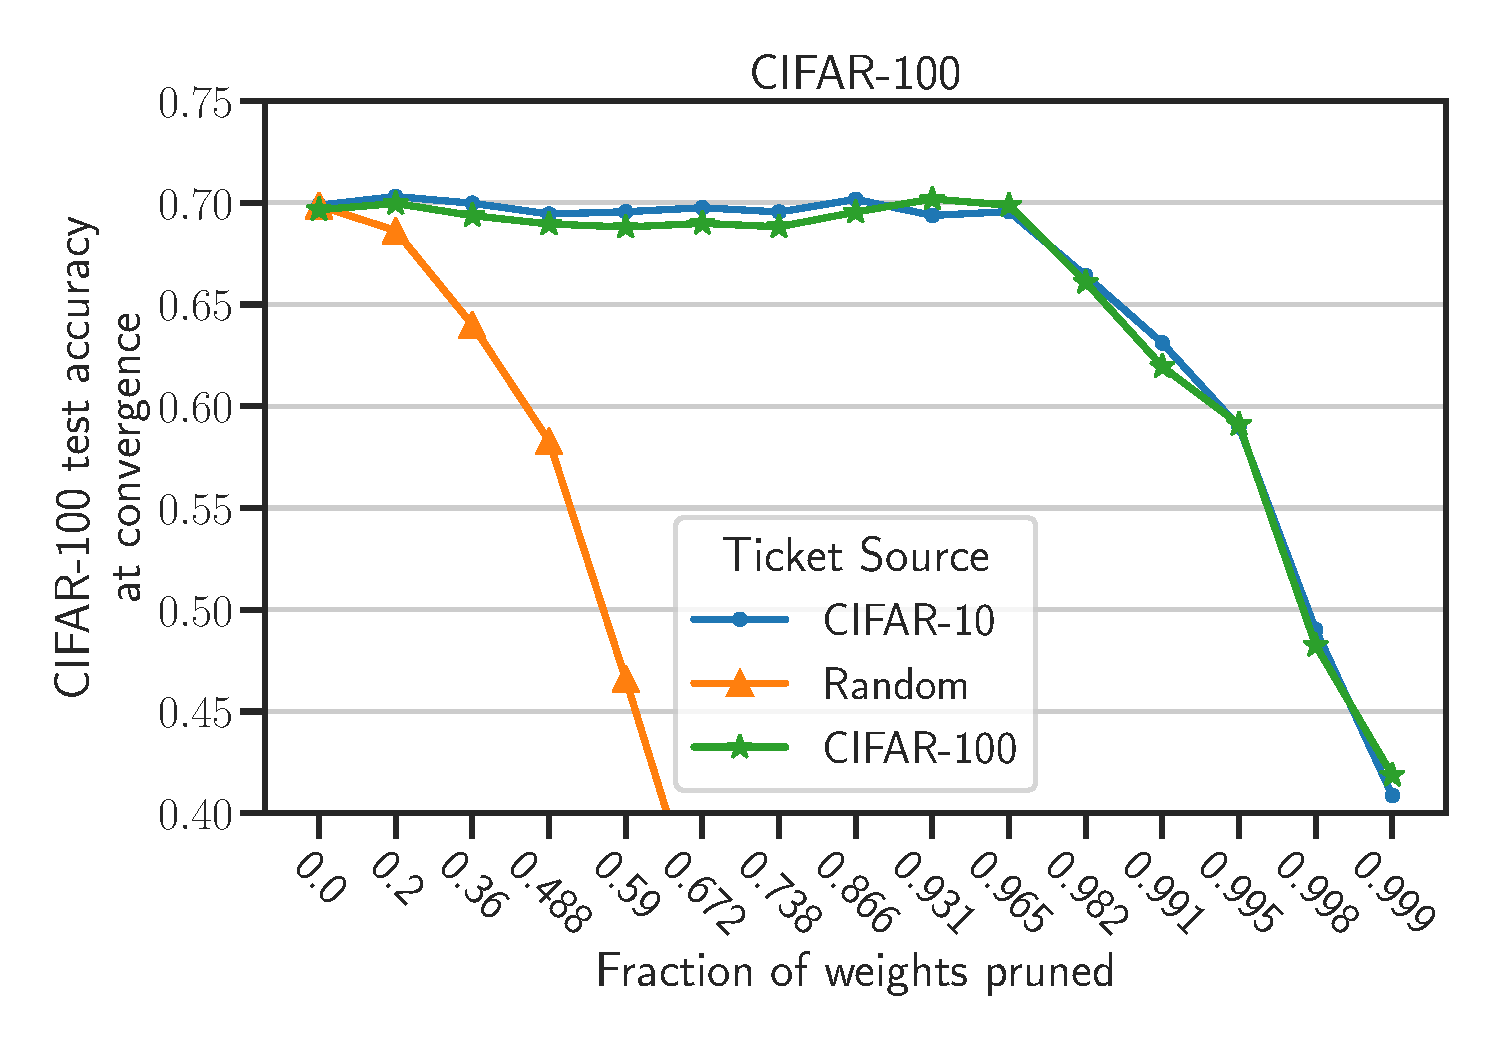
\includegraphics[width=\textwidth]{plots/Exp2_VGG_CIFAR100_N1.pdf}
    % \caption{Verifying transfer of winning ticket initializations across datasets - CIFAR100 with VGG19}
    % \label{fig:exp2_vgg_cifar100}
    \end{minipage}
%     \caption{Transfer of winning ticket initializations across datasets with VGG19}
%     \label{fig:exp2_vgg_1}
% \end{figure}
% \begin{figure}[h]
%     \centering
    \begin{minipage}{.497\textwidth}
   
    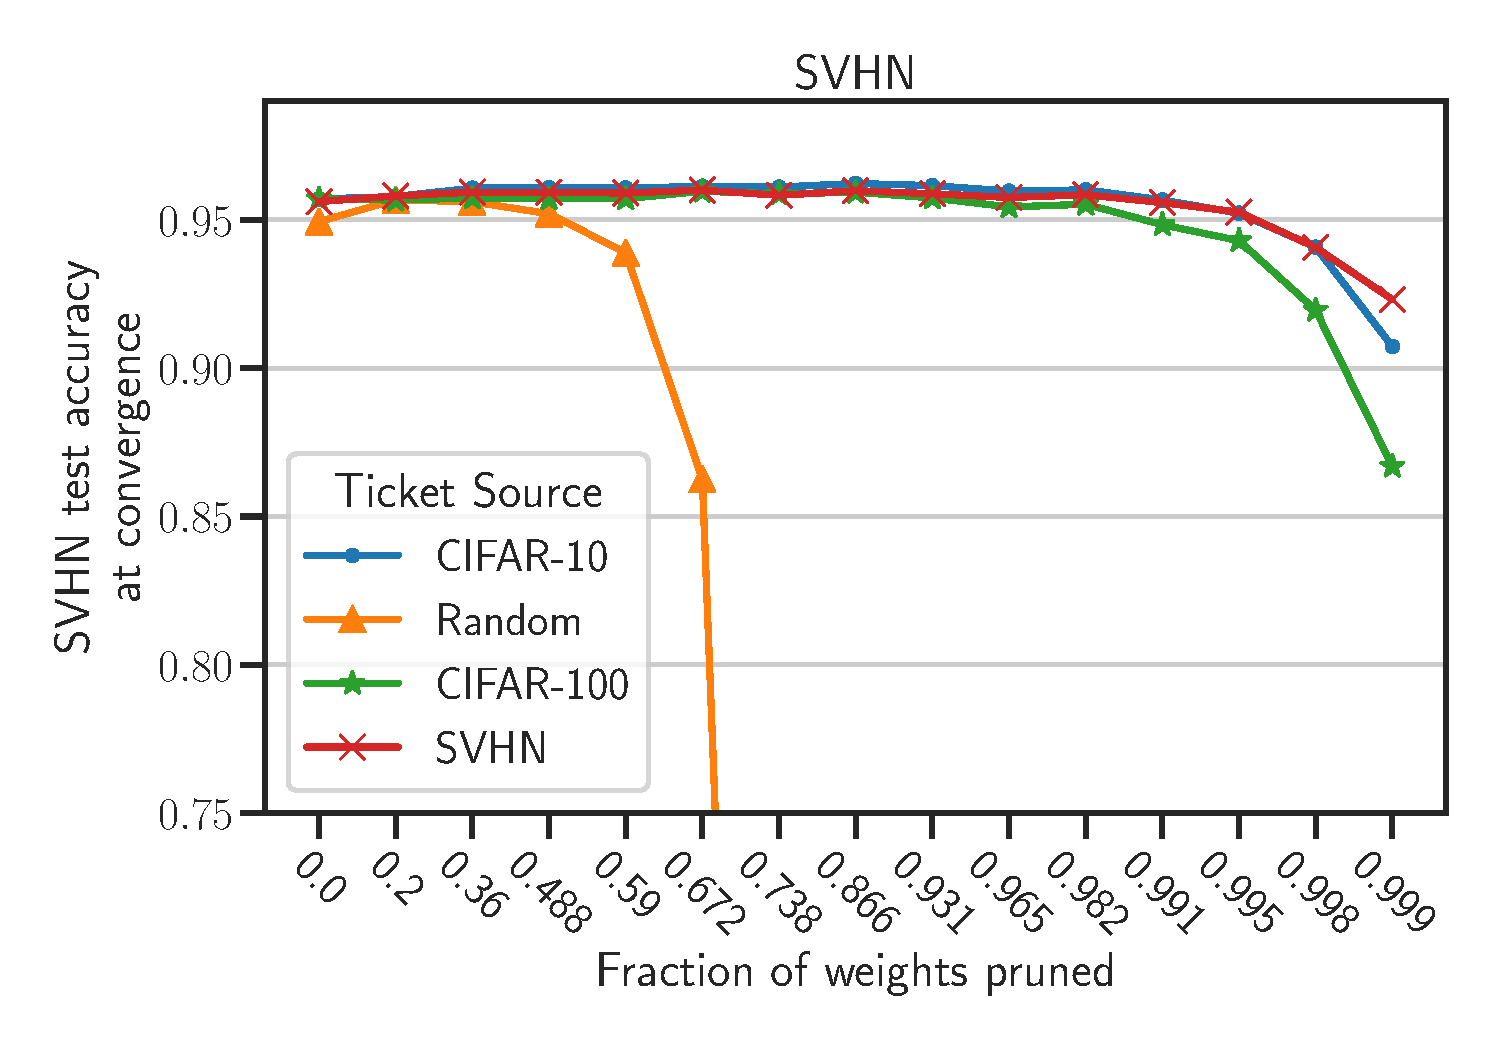
\includegraphics[width=\textwidth]{plots/Exp2_VGG_SVHN_N.pdf}
    % \caption{Verifying transfer of winning ticket initializations across datasets - SVHN with VGG19}
    % \label{fig:exp2_vgg_svhn}
    \end{minipage}
    \caption{Transfer of winning ticket initializations across datasets with VGG19}
    \label{fig:exp2_vgg}
\end{figure}

\subsection{Discussion}
 From our results, we make the following observations:
\begin{itemize}
    \item Winning ticket initializations transfer across multiple datasets and optimizers. This suggests that the winning tickets provide an inductive bias while training pruned models  and are not overfitting a particular optimizer or dataset.
    \item Winning tickets over more complex datasets(having more number of classes) generalize better to less complex datasets.
    \item  Different neural network architectures show different sensitivity to pruning fractions, with ResNet50 showing sharper accuracy degradation at higher pruning fractions than VGG19.
\end{itemize}
 Overall, these observations motivate further work in area of neural network initializations. Further, as generating lottery tickets using iterative pruning is computationally expensive and time-consuming, more efficient methods for generating winning tickets are needed.



\section{Conclusion}
The original paper \cite{repro_paper} investigates the generalizability of winning ticket initializations across datasets and optimizers. We replicate the experiments of the original paper from scratch. Our results support the major claims of the original paper and empirically show that the winning ticket initializations can be transferred across datasets and optimizers. We appreciate the authors' ability to explain their experiments and observations in a lucid and replicable manner. While the results are replicable, we find that process of reproducing the results is extremely compute-intensive. Hence along with our code base, we also open-source the winning tickets we find during our experiments.


\section{Acknowledgements}
We would like to thank Ari Morcos, Facebook AI Research for resolving our queries throughout this work. We would also like to thank Prof. Anirban Dasgupta, IIT Gandhinagar and Prof. Nipun Batra, IIT Gandhinagar for providing us Google Cloud credits for running the experiments. We would also like to thank the organizers of NeurIPS Reproducibility Challenge 2019 for providing us with CodeOcean credits. Further, we thank Mr. Rachit Chhaya, IIT Gandhinagar his comments on the report.


% \newpage
\bibliographystyle{ieeetr}


\bibliography{ref}

% References follow the acknowledgments. Use unnumbered first-level heading for
% the references. Any choice of citation style is acceptable as long as you are
% consistent. It is permissible to reduce the font size to \verb+small+ (9 point)
% when listing the references. {\bf Remember that you can use more than eight
%   pages as long as the additional pages contain \emph{only} cited references.}
% \medskip

% \small

% [1] Alexander, J.A.\ \& Mozer, M.C.\ (1995) Template-based algorithms for
% connectionist rule extraction. In G.\ Tesauro, D.S.\ Touretzky and T.K.\ Leen
% (eds.), {\it Advances in Neural Information Processing Systems 7},
% pp.\ 609--616. Cambridge, MA: MIT Press.

% [2] Bower, J.M.\ \& Beeman, D.\ (1995) {\it The Book of GENESIS: Exploring
%   Realistic Neural Models with the GEneral NEural SImulation System.}  New York:
% TELOS/Springer--Verlag.

% [3] Hasselmo, M.E., Schnell, E.\ \& Barkai, E.\ (1995) Dynamics of learning and
% recall at excitatory recurrent synapses and cholinergic modulation in rat
% hippocampal region CA3. {\it Journal of Neuroscience} {\bf 15}(7):5249-5262.

\end{document}
